\documentclass{beamer}
\usetheme{Singapore}
\usecolortheme{default}

\usepackage[utf8]{inputenc}
\usepackage[T1]{fontenc}
\usepackage{verbatim}
\usepackage{graphics}
\usepackage{listings}
\usepackage{lmodern}

\title{Understanding Git with Alloy}
\subtitle{Milestone 3}
\author{Cláudio Lourenço \and Renato Neves}
\institute{University of Minho\\
Formal Methods in Software Engineering}


\logo{ 
\includegraphics[width=0.15\textwidth]{images/csail_logo.png}
       
\includegraphics[width=0.15\textwidth]{images/uminho_eng_logo.png}}

\begin{document}

\frame {
   \titlepage
}

\frame{
   \frametitle{Table of contents}
   \tableofcontents 
}

\section{Git Structure}
\begin{frame}
   \frametitle{The Git Structure}
   \begin{figure}
      \centering
      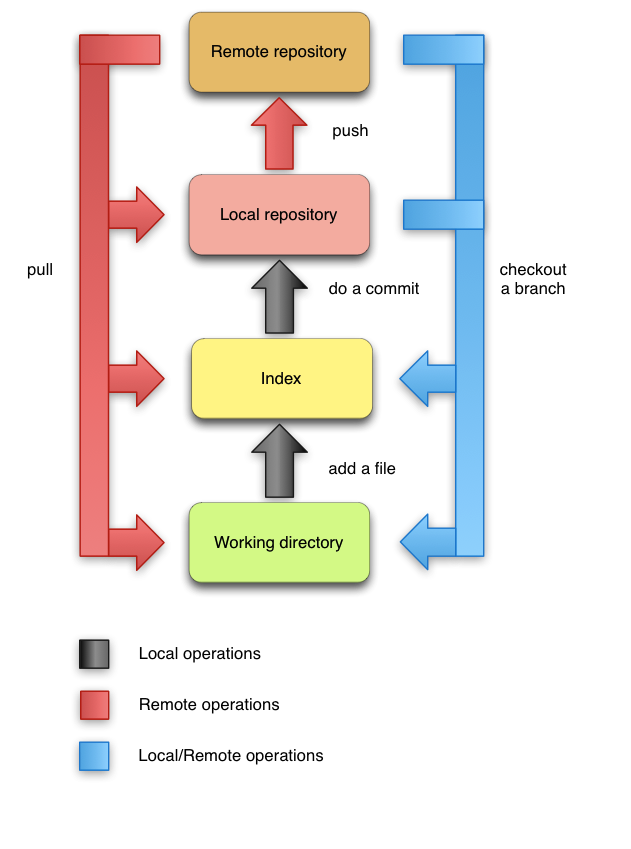
\includegraphics[width=0.5\textwidth]{images/git_workflow.png}
   \end{figure}
\end{frame}

\section{Repository}
\begin{frame}
   \frametitle{Repository}
   \begin{centering}
      \begin{itemize}
         \item Objects
            \begin{itemize}
               \item Blob;
               \item Tree;
               \item Commit;
               \item Tag;
            \end{itemize}
         \item References
            \begin{itemize}
               \item Branch;
               \item HEAD;
            \end{itemize}
      \end{itemize}
   \end{centering}
\end{frame}

\begin{frame}
   \frametitle{Blob and Tree}
   \begin{block}{Blob}
      \begin{itemize}
         \item Represents the content of a file;
         \item The name is calculated on its content;
      \end{itemize}
   \end{block}
      \tiny
      \begin{lstlisting}
      sig Blob extends Object {}
      \end{lstlisting}
\end{frame}

\section{Working Directory}
\begin{frame}
   \frametitle{Working Directory}
\end{frame}

\section{Index}
\begin{frame}
   \frametitle{Index}
\end{frame}

\section{Operations}
\begin{frame}
   \frametitle{Operations}
\end{frame}

\end{document}
